\subsubsection{Dynamiske side af analysen}
\textbf{Opret sag}\\
Beskrivelse:\\
Som man kan se på figur \ref{fig:opretSag} startes opret sag ved at en aktør anmoder systemet om at oprette en sag. 
Afdelingen håndterer operationen ved at hente en formular ved at sende forespørgsel til Sag. 
Den sender sagsåbningsformularen tilbage til afdeling. Når afdelingen modtager formularen, videresendes den til den pågældende aktør. Aktøren udfylder formularen med relevante oplysninger, hvorefter den sendes til afdelingen, hvor denne sender det videre til den pågældende sag for opdatering. \\
\begin{figure}[htb!]
  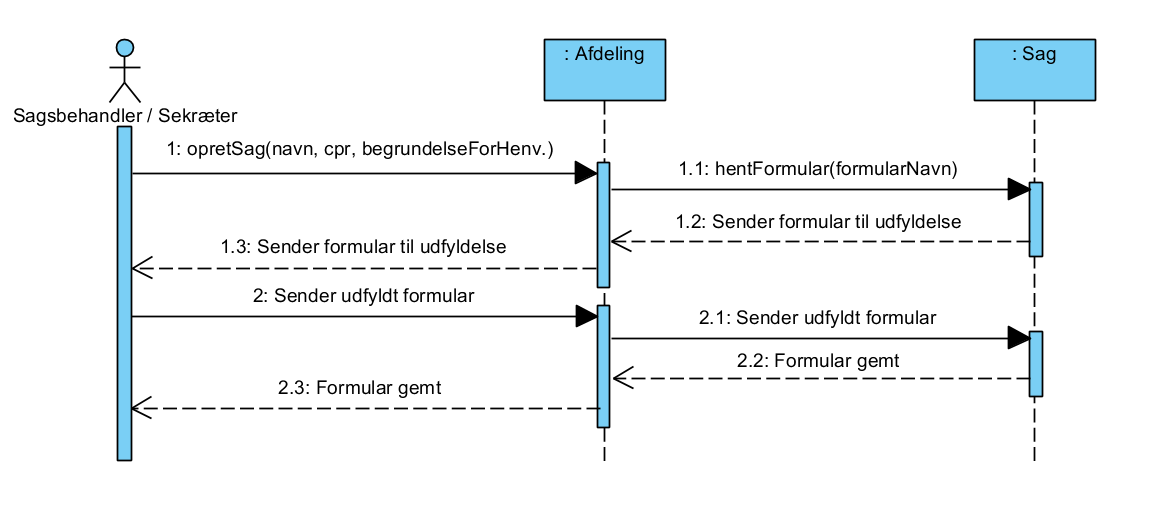
\includegraphics[width=\linewidth]{./PNG/analyse/opretSag.PNG} 
  \caption{Sekvensdiagram for opret sag}
  \label{fig:opretSag}
\end{figure}\\
\textbf{Find sag} \label{af:findSag}\\
Beskrivelse: \\
En aktør, f.eks. sagsbehandler eller sekretær, vælger at søge på en sag, som vist i figur \ref{fig:findSag}. Search metoden modtager en nøgle værdi. Den sender besked ned til afdelingen og herefter spørger en metode efter at finde alle sager med den specifikke nøgleværdi. Sager med den specifikke nøgle sendes tilbage til afdelingen og afdelingen sender resultatet videre til aktøren. Herefter vælger aktøren at åbne den specifikke sag, hvor der kaldes på openCase metoden som sender besked ned til afdelingen. Afdelingen efterspørger herefter om at få den sag med det specifikke sagsnummer, og der returneres et sagsobjekt med det specifikke sagsnummer. Afdeling returnerer efterfølgende det fundne sagsobjekt til aktøren. \\ \\
\begin{figure}[htb!]
  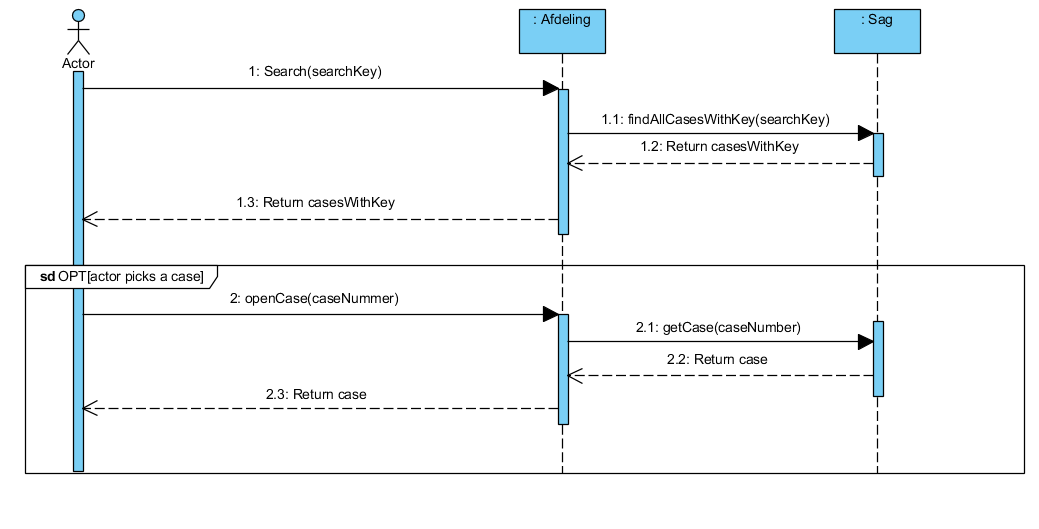
\includegraphics[width=\linewidth]{./PNG/analyse/findSag.PNG} 
  \caption{Sekvensdiagram for find sag}
  \label{fig:findSag}
\end{figure}